% ============================================================
%  Figure 1 — (a) Kairos pipeline | (b) per-endpoint weights
%             heatmap + fitting objective + stacked composition
%  Native width ~ 16.4 cm == \linewidth, inserted 1:1.
%  Build: pdflatex fig_kairos_arch.tex
% ============================================================
\documentclass[border=3pt]{standalone}
\usepackage{tikz}
\usepackage{amsmath,amssymb}
\usetikzlibrary{arrows.meta, calc}

\definecolor{boxblue}{HTML}{E8EEF7}
\definecolor{boxamber}{HTML}{FDF3DC}
\definecolor{boxpink}{HTML}{FBE9E9}
\definecolor{accent}{HTML}{3F6399}
\definecolor{accb}{HTML}{7C9BC4}
\definecolor{accc}{HTML}{A8BDD6}
\definecolor{accd}{HTML}{CCD8E8}
\definecolor{acce}{HTML}{E4EAF3}
\colorlet{bd}{black!65}

\tikzset{
  comp/.style={rounded corners=2pt, draw=bd, line width=0.5pt, fill=#1,
               inner sep=2pt, align=center, font=\scriptsize,
               text width=2.85cm, minimum height=1.05cm},
  comp/.default=boxblue,
  ar/.style={-{Stealth[length=1.4mm,width=1.0mm]}, line width=0.55pt,
             black!72, shorten >=0.3mm},
}

\begin{document}
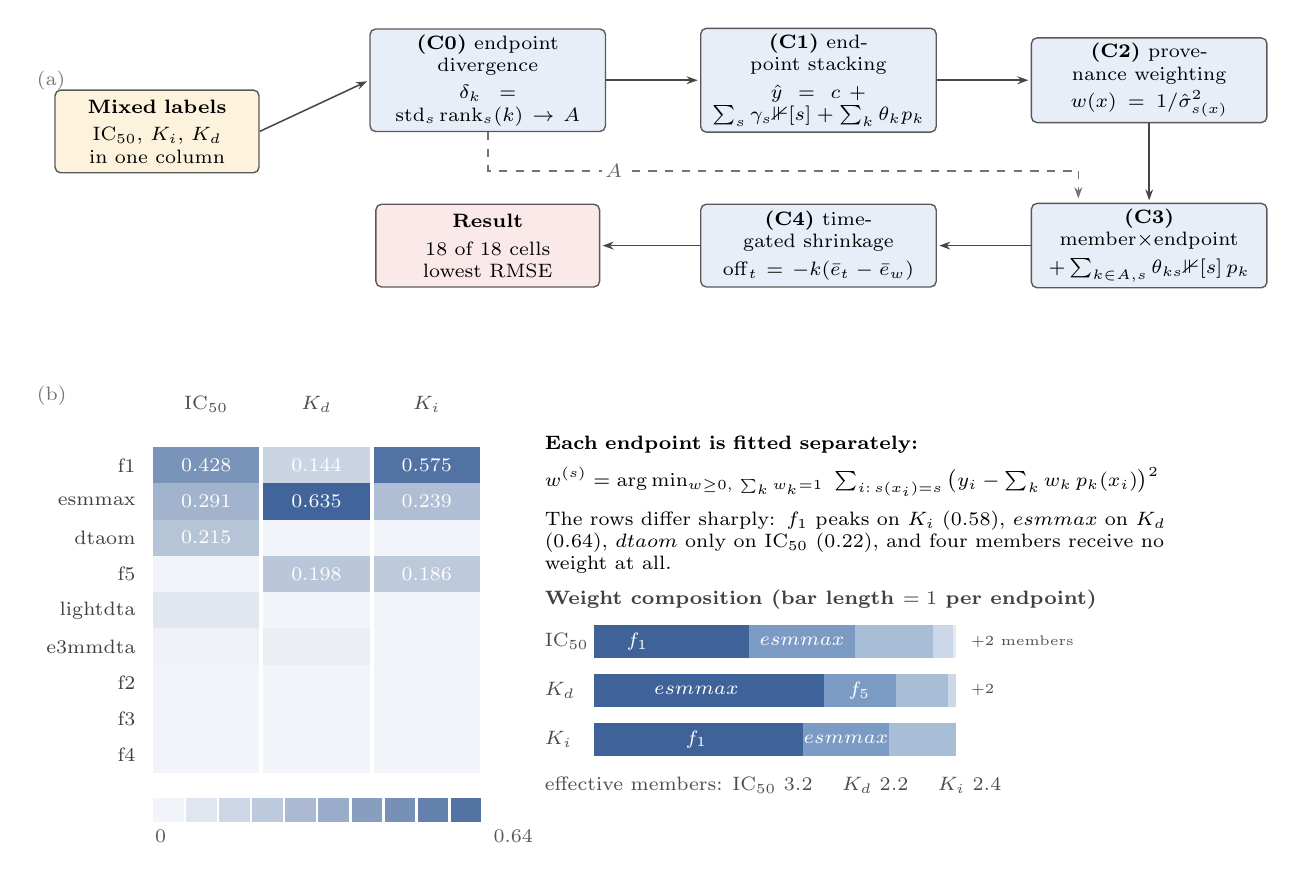
\begin{tikzpicture}

% ============================================================
%  (a) pipeline — spans the full width
% ============================================================
\node[font=\scriptsize, black!55, anchor=west] at (0.15, 3.95) {(a)};

\node[comp, fill=boxamber, text width=2.45cm] (P) at (1.80, 3.30)
  {\textbf{Mixed labels}\\[2pt]
   {\scriptsize IC$_{50}$, $K_i$, $K_d$ in one column}};

\node[comp] (c0) at (6.00, 3.95)
  {\textbf{(C0)} endpoint divergence\\[2pt]
   {\scriptsize $\delta_k=\mathrm{std}_s\,\mathrm{rank}_s(k)\rightarrow A$}};
\node[comp] (c1) at (10.20, 3.95)
  {\textbf{(C1)} endpoint stacking\\[2pt]
   {\scriptsize $\hat y=c+\sum_s\gamma_s\mathbb 1[s]+\sum_k\theta_k p_k$}};
\node[comp] (c2) at (14.40, 3.95)
  {\textbf{(C2)} provenance weighting\\[2pt]
   {\scriptsize $w(x)=1/\hat\sigma^2_{s(x)}$}};
\node[comp] (c3) at (14.40, 1.85)
  {\textbf{(C3)} member$\times$endpoint\\[2pt]
   {\scriptsize $+\sum_{k\in A,s}\theta_{ks}\mathbb 1[s]\,p_k$}};
\node[comp] (c4) at (10.20, 1.85)
  {\textbf{(C4)} time-gated shrinkage\\[2pt]
   {\scriptsize $\mathrm{off}_t=-k(\bar e_t-\bar e_w)$}};
\node[comp, fill=boxpink, text width=2.70cm] (R) at (6.00, 1.85)
  {\textbf{Result}\\[2pt]
   {\scriptsize 18 of 18 cells lowest RMSE}};

\draw[ar] (P.east) -- (c0.west);
\draw[ar] (c0.east) -- (c1.west);
\draw[ar] (c1.east) -- (c2.west);
\draw[ar] (c2.south) -- (c3.north);
\draw[ar] (c3.west) -- (c4.east);
\draw[ar] (c4.west) -- (R.east);
% C0 -> C3 : subset A (orthogonal, enters C3 from the top)
\draw[dashed, black!55, line width=0.55pt]
  (c0.south) -- (6.00,2.80) -- (13.50,2.80);
\draw[ar, dashed, black!55, line width=0.55pt] (13.50,2.80) -- (13.50,2.42);
\node[font=\scriptsize, text=black!60, fill=white, inner sep=1.2pt]
  at (7.6,2.80) {$A$};

% ============================================================
%  (b) heatmap (left) | objective + stacked composition (right)
% ============================================================
\node[font=\scriptsize, black!55, anchor=west] at (0.15, -0.05) {(b)};

% ---------- heatmap: 9 members x 3 endpoints ----------
\begin{scope}[shift={(1.75, -0.45)}]
  \foreach \ep/\col in {IC$_{50}$/0,$K_d$/1,$K_i$/2}{%
    \node[font=\scriptsize, black!70, anchor=south]
      at ({1.40*\col+0.675},0.06) {\ep};}
  \foreach \mem/\a/\b/\c/\r in {%
    f1/0.428/0.144/0.575/0,%
    esmmax/0.291/0.635/0.239/1,%
    dtaom/0.215/0/0/2,%
    f5/0/0.198/0.186/3,%
    lightdta/0.056/0.001/0/4,%
    e3mmdta/0.010/0.022/0/5,%
    f2/0/0/0/6,f3/0/0/0/7,f4/0/0/0/8}{%
    \pgfmathsetmacro\ytop{-0.46*\r-0.26}
    \pgfmathsetmacro\ymid{\ytop-0.23}
    \node[font=\scriptsize, black!75, anchor=east] at (-0.10,\ymid) {\mem};
    \foreach \col/\v in {0/\a,1/\b,2/\c}{%
      \pgfmathsetmacro\op{0.07+0.92*\v/0.635}
      \fill[accent, opacity=\op]
        ({1.40*\col},\ytop) rectangle ++(1.35,-0.46);
      \pgfmathparse{\v>0.09?1:0}
      \ifnum\pgfmathresult=1
        \node[font=\scriptsize, white] at ({1.40*\col+0.675},\ymid) {\v};
      \fi
    }
  }
  \foreach \i in {0,...,9}{%
    \pgfmathsetmacro\op{0.07+0.092*\i}
    \fill[accent, opacity=\op] ({0.42*\i},-4.72) rectangle ++(0.39,-0.30);
  }
  \node[font=\scriptsize, black!65, anchor=west] at (-0.10,-5.20) {0};
  \node[font=\scriptsize, black!65, anchor=west] at (4.20,-5.20) {0.64};
\end{scope}

% ---------- fitting objective ----------
\node[anchor=north west, text width=8.5cm, align=left, font=\scriptsize]
  at (6.60, -0.45)
  {\textbf{Each endpoint is fitted separately:}\\[4pt]
   $w^{(s)}=\arg\min_{w\ge 0,\ \sum_k w_k=1}\
    \sum_{i:\,s(x_i)=s}\big(y_i-\sum_k w_k\,p_k(x_i)\big)^2$\\[4pt]
   The rows differ sharply: $f_1$ peaks on $K_i$ ($0.58$), $esmmax$ on $K_d$
   ($0.64$), $dtaom$ only on IC$_{50}$ ($0.22$), and four members receive no
   weight at all.};

% ---------- stacked composition per endpoint ----------
% left edge aligned with the objective text above (x = 6.60)
\begin{scope}[shift={(7.35, -2.95)}]
  \node[font=\scriptsize, black!75, anchor=west] at (-0.75, 0.30)
    {\textbf{Weight composition (bar length $=1$ per endpoint)}};
  % ---- IC50 : total bar 4.6 cm ----
  \node[font=\scriptsize, black!70, anchor=west] at (-0.75,-0.23) {IC$_{50}$};
  \fill[accent]  (0,-0.44) rectangle (1.97,-0.02);
  \fill[accb]    (1.97,-0.44) rectangle (3.31,-0.02);
  \fill[accc]    (3.31,-0.44) rectangle (4.30,-0.02);
  \fill[accd]    (4.30,-0.44) rectangle (4.56,-0.02);
  \fill[acce]    (4.56,-0.44) rectangle (4.60,-0.02);
  \node[font=\scriptsize, white] at (0.55,-0.23) {$f_1$};
  \node[font=\scriptsize, white] at (2.64,-0.23) {$esmmax$};
  \node[font=\tiny, black!70, anchor=west] at (4.66,-0.23) {$+2$ members};
  % ---- Kd ----
  \node[font=\scriptsize, black!70, anchor=west] at (-0.75,-0.85) {$K_d$};
  \fill[accent]  (0,-1.06) rectangle (2.92,-0.64);
  \fill[accb]    (2.92,-1.06) rectangle (3.83,-0.64);
  \fill[accc]    (3.83,-1.06) rectangle (4.49,-0.64);
  \fill[accd]    (4.49,-1.06) rectangle (4.60,-0.64);
  \node[font=\scriptsize, white] at (1.30,-0.85) {$esmmax$};
  \node[font=\scriptsize, white] at (3.37,-0.85) {$f_5$};
  \node[font=\tiny, black!70, anchor=west] at (4.66,-0.85) {$+2$};
  % ---- Ki ----
  \node[font=\scriptsize, black!70, anchor=west] at (-0.75,-1.47) {$K_i$};
  \fill[accent]  (0,-1.68) rectangle (2.65,-1.26);
  \fill[accb]    (2.65,-1.68) rectangle (3.75,-1.26);
  \fill[accc]    (3.75,-1.68) rectangle (4.60,-1.26);
  \node[font=\scriptsize, white] at (1.30,-1.47) {$f_1$};
  \node[font=\scriptsize, white] at (3.20,-1.47) {$esmmax$};
  % effective member count
  \node[font=\scriptsize, black!70, anchor=west] at (-0.75,-2.05)
    {effective members: IC$_{50}$ $3.2$ \quad $K_d$ $2.2$ \quad $K_i$ $2.4$};
\end{scope}

\end{tikzpicture}
\end{document}